\documentclass[11pt]{article}
\usepackage{amsmath, amssymb, amsthm}
\usepackage{graphicx}
\usepackage{geometry}
\geometry{margin=1in}
\usepackage{hyperref}
\usepackage{graphicx}
\usepackage{pgfplots}
\pgfplotsset{compat=1.18} % or newer if available



% Title with math formatting
\title{R2 andre kapittel}
\author{Martino}
\date{\today}

\begin{document}

\maketitle

\begin{abstract}
  xd
\end{abstract}

\section{Introduction}


\begin{theorem}
  xd
\end{theorem}

\begin{proof}
  test
\end{proof}

\section{Numerisk derivasjon}
\begin{center}
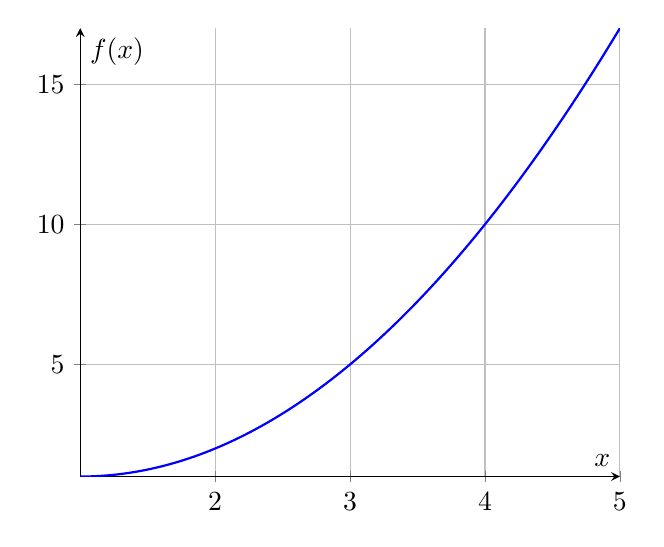
\begin{tikzpicture}
  \begin{axis}[
    axis lines = middle,
    xlabel = $x$,
    ylabel = {$f(x)$},
    grid=major,
    samples=100,
    domain=1:5
  ]
    \addplot [blue, thick] {x^2-2*x+2};
  \end{axis}
\end{tikzpicture}
\end{center}
Vi bruker at:
\begin{equation}
\int_a^b f(x)dx\approx\sum_{i=1}^n f(x_{i-1})\cdot \Delta x \quad \text{der} \quad x_{i-1}=a+(i-1)\cdot\Delta x \qquad
  \label{eq:}
\end{equation}

\begin{figure}[h!]
  \centering
  \includegraphics[width=0.6\textwidth]{assets/numerisk_derivasjon.png}
  \caption{Implementering av numerisk derivasjon i \textit{python}. Konsoll: \texttt{7.999199919991998}}
  \label{fig:sample-image}
\end{figure}
\end{document}
